\section{Theory}
\label{sec:theory}
In this section, several related works are discussed including properties of
gossip algorithm and gossip-based aggregation algorithm. One example of
aggregation is described in details to illustrate how massage exchanges are
performed, along with the explanation of pull-push based pseudo code. Number of
link is chosen as the attribute for our condition control experiments. Reasons
of analysing real networks are stated and based upon these facts we derive our
hypothesis.

\subsection{Related work}
Motivated by peer-to-peer and ad hoc networks, a considerable number of studies have been done regarding gossip-based algorithms. Convergence and upper bound consensus time have been proven by J.Lavaei and R.Murray in \cite{5929538}. Analytical methods and simulations have been utilized to examine the relations between performance of gossip protocols and topology of network, namely randomness, connectivity etc. As a subcategory of distributed algorithm different models, such as synchronous and asynchronous models, with or without churn, are discussed in \cite{Lynch:1996:DA:525656}. The optimization of parameters of an asynchronous randomized gossip algorithm for faster convergence is proven to be a semi-definite problem \cite{Boyd2004}.

Our study is mainly based on the work of M.Jelasity, A.Montresor and O.Babaoglu \cite{jelasity_gossip-based_2005}, focusing on existing static networks of different topologies \cite{knight_internet_2011}

\subsection{Gossip-based aggregation}
Gossip algorithm as a branch of distributed algorithm, denotes an message exchange and dissemination mechanism in a decentralised manner. Gossip-based aggregation is a data collection and message propagation method based on this algorithm.
%TODO: describe the algorithm in details
\subsubsection{Gossip algorithm}
To better understand of gossip algorithm, we assume a graph as in figure \ref{fig:epochs}. It illustrates a typical message dissemination process applying gossip algorithm. It starts with one node containing the information to be propagated, as in subgraph (a). It randomly chooses one neighbor and send the message. In second epoch, as showed in subgraph (b), this message is  forwarded to next hop in the same manner, including the root node. By recursively applying same procedures, the message will be spread through the whole network. Subgraph (c) shows the occurrence of probable redundant packet from node 3 to node 2, in which the message was acquired before. Due to the randomness of gossip algorithm, complete dissemination can only be achieved with a certain probability within given epochs, which can be denoted as $D(x)=\int_0^x P(\xi)\mathrm{d}\xi$
\begin{figure}[h!]
   \begin{subfigure}[t]{0.45\textwidth}
      \vspace{0pt}
      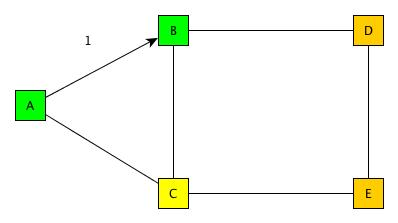
\includegraphics[width=\linewidth]{figures/network_gossip_1.jpg}
      \caption{Beginning of message dissemination}
   \end{subfigure}
   \hfill
   \begin{subfigure}[t]{0.45\textwidth}
      \vspace{0pt}
      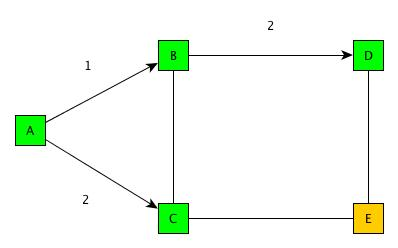
\includegraphics[width=\linewidth]{figures/network_gossip_2.jpg}
      \caption{Passing the message}
   \end{subfigure}
   \vspace{2ex}
     \begin{center}
     \begin{subfigure}[c]{0.45\textwidth}
      \vspace{0pt}
      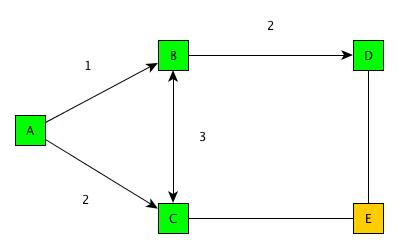
\includegraphics[width=\linewidth]{figures/network_gossip_3.jpg}
      \caption{Probable redundant message}
   	\end{subfigure}
   \end{center}
   \caption{Gossip algorithm evolution epochs}
   \label{fig:epochs}
\end{figure}

\subsubsection{Aggregation}
% TODO: illustrate aggregation
Listing \ref{code:pseudo} shows a simple implementation of synchronous gossip-based aggregation algorithm, inspired by \cite{jelasity_gossip-based_2005}.
\begin{figure}[!h]
\begin{lstlisting}[caption={Pseudo Code for gossip-based aggregation}, label=code:pseudo, mathescape=true, captionpos=b]
$ActiveGossipThread$
$\mbox{for each consecutive } \delta \mbox{ time units at randomly picked time; do}$
    $q \leftarrow GET\_NEIGBOR()$
    $send\_to({state}_{p},$ $q)$
    $state_{q} \leftarrow receive(q)$
    $state_{p} \leftarrow UPDATE(state_{p},$ ${state}_{q})$

$PassiveGossipThread$
$\mbox{while true:}$
    $state_{q} \leftarrow receive(*)$
    $send\_to(state_{p},$ $q)$
    $state_{p} \leftarrow UPDATE(state_{p},$ $state_{q})$
\end{lstlisting}
\end{figure}

Although convergence is proven and expected convergence time can be estimated by probability density function for a certain topology \cite{5929538}, a drawback of probabilistic algorithm is reliability \cite{Lynch:1996:DA:525656}, when compared to deterministic. The value can only be considered as true result with a certain probability. To put this protocol into practice, some extra procedures need to be added. In this study, we leave out the correctness check inside implementation but try to obtain an empirical criteria according to the result of experiments.

\subsection{Impact of topology on the performance of aggregation}
Plenty of methods exist to describe overlay topologies of a network, and different representations are used to describe properties of a topology. Moreover, the performance of gossip-based aggregation is also abstracted differently for specific purpose.

In this study, we focus on investigating the relation between performance of convergence and number of links of a given set of topologies. 

\subsection{Applying to real network}
In order to apply control variable experiment method, we based our experiment on 4 real network topologies (see figure \ref{fig:graphs}) with same number of nodes (37) and different number of links, as shown in Table \ref{table:network}.

\begin{figure}[h!]
   \begin{minipage}[t]{0.4\textwidth}
      \vspace{0pt}
      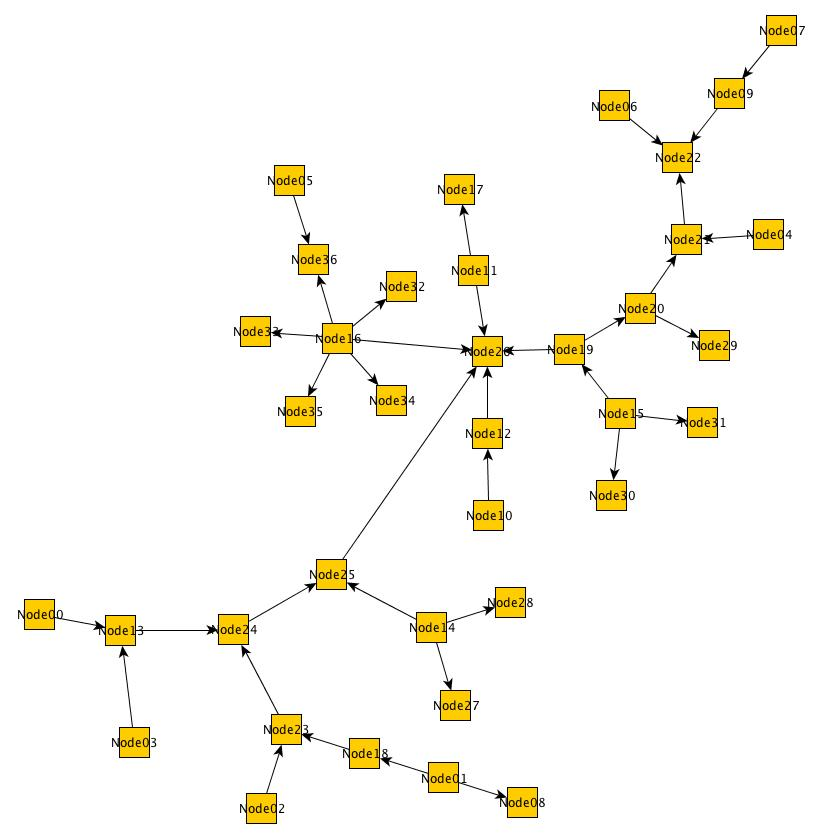
\includegraphics[width=\linewidth]{Reuna.jpg}
      Backbone of Chile (a)
   \end{minipage}
   \hfill
   \begin{minipage}[t]{0.4\textwidth}
      \vspace{0pt}
      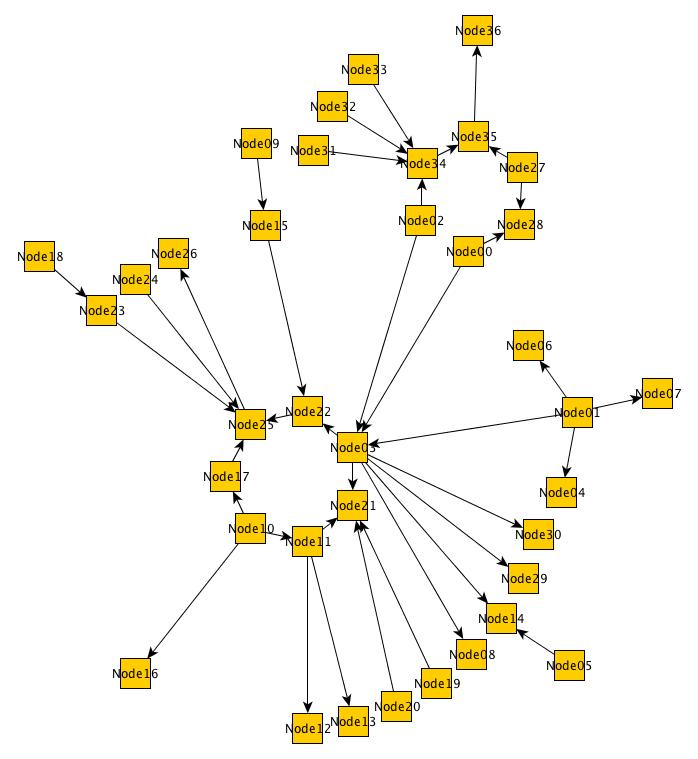
\includegraphics[width=\linewidth]{Bren.jpg}
      Backbone of Bulgaria (b)
   \end{minipage}
   \vspace{4ex}
    \begin{minipage}[c]{0.45\textwidth}
    \vspace{0pt}
    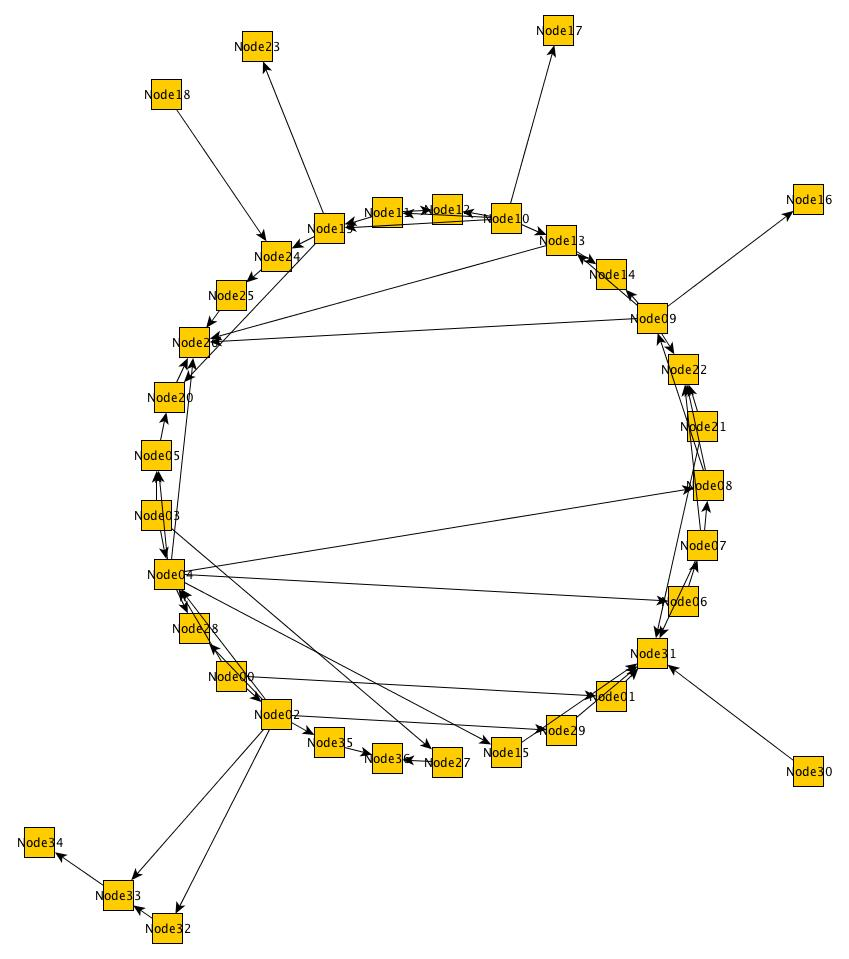
\includegraphics[width=\linewidth]{Geant2010.jpg}
    European transit network (c)
    \end{minipage}
    \begin{minipage}[c]{0.4\textwidth}
    \vspace{0pt}
    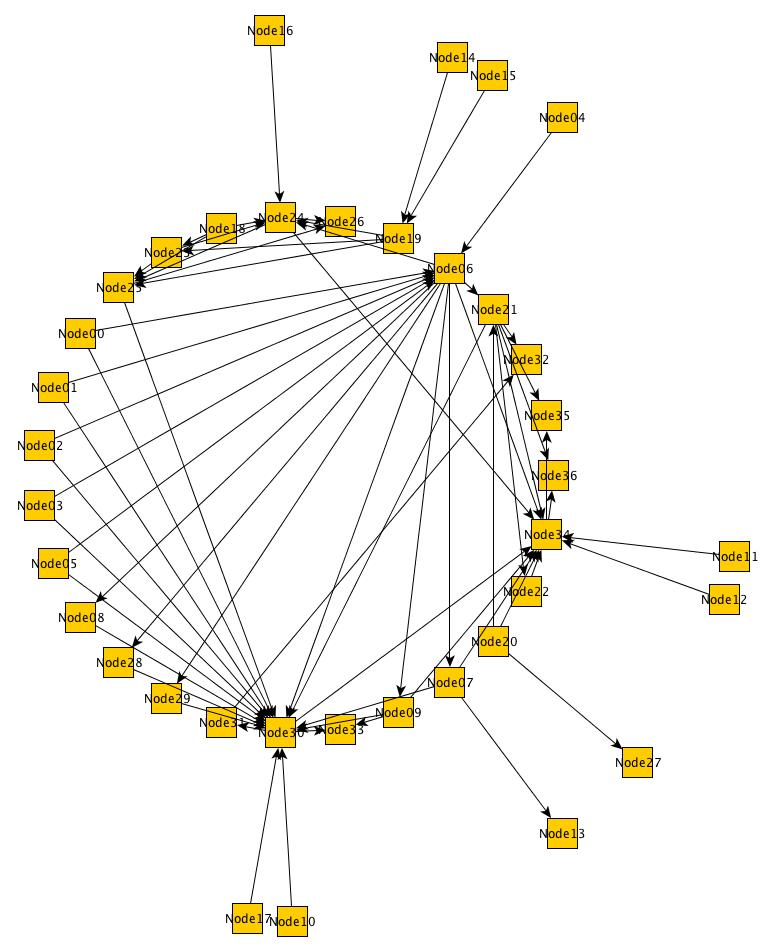
\includegraphics[width=\linewidth]{Iij.jpg}
    Backbone network Japan, USA (d)
    \end{minipage}
   \caption{Different graph topologies (in ring layout)}
   \label{fig:graphs}
\end{figure}
\begin{table}
\centering
\caption{Topologies under investigation}
\begin{tabular}{lrrcrr}
	\hline
	Name of Network & Year & Country & \# of Links\\% & Entropy1 & Entropy2\\
    \hline
    Reuna & 2010 & Chile & 36\\% & 202.0476 & 0.5164084\\
    BREN & 2010 & Bulgaria & 38\\% & 210.2229 & 0.6214745\\
    Geant & 2010 & Europe & 58\\% & 277.3282 & 1.530375\\
    Iij & 2010 & Japan, USA & 66\\% & 307.2482 & 1.553654\\
    \hline
\end{tabular}
\label{table:network}
\end{table}

\subsection{Hypothesis}
%{\it Hypothesis 1.}
In a given network topology $\mathcal{G}=\{\mathcal{E}, \mathcal{V}\}$, the number of links (edges) $N_E$ and convergence time $t$ are positively correlated, with number of nodes (vertices) $N_V$ unchanged.
%{\it Hypothesis 2.} In a given network topology $\mathcal{G}=\{\mathcal{E}, \mathcal{V}\}$, the entropy of this graph $S$ and convergence time $t$ are positively correlated.

\subsection{Research methodology and methods}
We apply a positivistic investigation grounded in quantitative experiments. With induction in the form of statistical inference, we aim to predict the behavior of the system under question in the boundary of our experimental research.
%Not quite sure about this expression
%One paragraph or many little paragraphs

We clearly distinguish our study from realism, as we use network graphs inspired by real networks, but leave it to other research to prove that the experiment is representative of those real networks.

Since we will investigate several existing networks with the same number of nodes (constant) but different number of links (variable), we choose experimental research as our research method.

We will apply inductive reasoning research approach to verify the hypothesis. Since our unique contribution is an investigation of real network rather than a theoretical proof, deductive reasoning research approach does not fit our goal.
